%!TEX root = ../Thesis.tex

\chapter{Speaker diarization} \label{ch:chap2}

\epigraphhead[70]{
\epigraph{I thank you for your voices: thank you:
Your most sweet voices.}{William Shakespeare}}
 
Se conoce como \SD~ al problema de segmentación automática de audio a partir de la identificación de las diferentes personas que participan en una grabación. Esto se realiza generalmente identificando los segmentos que son más \textit{homogéneos} y a partir de estos, identificar el número de personas que hablan en la grabación.

Se considera que cada persona posee ciertas características propias que la diferencian de los demás. Por ejemplo, tanto la tesitura como el timbre son rasgos que varían de persona a persona.

La idea básica cuando se busca abordar este problema es el de poder segmentar la señal de audio de acuerdo a los cambios que ocurren en ésta. Es decir, detectar por ejemplo las variaciones en la voz (que usualmente implican que alguien más está hablando) y luego, con todos los segmentos obtenidos, tratar de agruparlos según características similares; pues una misma persona tiene características propias en su voz. 

\section{Aplicaciones de \sd}

Por la misma naturaleza del problema, cuando se realiza \sd, lo que se trata de inferir es cuántas personas hablan, y en qué momentos habla cada una de ellas; es decir, se identifica a un grupo $n$ de personas, pero no se dice nada acerca de ellos o su identidad. 

Debido a esto, las etiquetas asignadas a cada persona identificada en la grabación puede cambiar, pues no hay nada que nos permita asociar de manera no arbitraria una etiqueta a una persona en especifico. Es decir, el orden en que se asignan las etiquetas puede cambiar, aunque la segmentación obtenida sea en esencia la misma.

La segmentación y agrupación de voz, es una parte importante de la transcripción de voz, así como también del reconocimiento de voz e identificación de personas que hablan. 

Es de gran ayuda para la tarea de reconocimiento de voz, puesto que éste se basa en identificar palabras completas; por lo que al lograr segmentar una señal de audio de acuerdo a las personas que hablan, se tendrá entonces muy seguramente una buena segmentación tanto de palabras como oraciones completas.

En cuanto a la identificación de personas y alguna otra modelación acústica que se quiera realizar; es importante que los modelos que se entrenan usen segmentos de audio homogéneos (en este caso, que se tenga la certeza que corresponden a la misma persona), para que en realidad se esté modelando la voz de la persona, y no algo diferente a ella.

Como último ejemplo, la transcripción automática de voz, es el proceso en el que además de lograr identificar cuándo habla cada persona, se identifica de quién se trata realmente esta persona, y qué es lo que está diciendo. Ésto sirve por ejemplo, cuando se tiene una gran cantidad de grabaciones de audio; y se desea etiquetar de qué se habla en cada una de estas grabaciones. 

\section{Formulación matemática}

De forma general, se esbozará cuál es el problema que trata de resolver con \sd. El enfoque que se usará es estadístico, entonces en la formulación es necesario el cálculo de probabilidades. 

Denótese por $\mathcal{A}$ la evidencia acústica o los datos a partir del cuál el modelo deberá encontrar la segmentación correcta para un fragmento de señal. Sin entrar mucho a detalle, y puesto que de alguna manera se debe digitalizar y caracterizar la señal analógica de audio; podemos pensar en $\mathcal{A}$ como la secuencia de símbolos correspondiente a un segmento de señal, y que está conformada por elementos de un alfabeto mucho más grande $\mathbb{A}$. 
\begin{equation}
\mathcal{A} = a_1, a_2, ..., a_K \quad a_i \in \mathbb{A}
\label{eqn:2a-1}
\end{equation}
en donde los sub-índices de los elementos $a_i$ hacen referencia a un intervalo de tiempo $i$ en la secuencia de audio original, y los valores que tomen pueden repetirse de acuerdo a la grabación.

De la misma manera, definamos 
\begin{equation}
\mathcal{S} = s_1, s_2, ..., s_N \quad s_i \in \mathbb{S}
\label{eqn:2a-2}
\end{equation}
donde $\mathcal{S}$ es la secuencia que corresponde a la segmentación correcta para un intervalo del audio original. En este caso $\mathbb{S}$ es el conjunto de todos los interlocutores que participan en la grabación de audio y que por el momento se considerará como información conocida; y $s_i$ de igual manera representa al interlocutor que habla en el tiempo $i$.

Si $P(\mathcal{S} \,|\, \mathcal{A})$ denota la probabilidad de que una secuencia de interlocutores $\mathcal{S}$ esté hablando dada la evidencia acústica en $\mathcal{A}$, entonces una forma de escoger cuáles son los personas que hablan en ese intervalo se puede calcular de la siguiente manera:
\begin{equation}
\hat{\mathcal{S}} = \underset{\mathcal{S}}{arg~max}~ P(\mathcal{S} \,|\, \mathcal{A})
\label{eqn:2a-3}
\end{equation}
Esto es, se seleccionaría la sucesión de interlocutores más probable para una secuencia de datos dada.

Por el teorema de Bayes, podemos reescribir la parte derecha de \eqref{eqn:2a-3} como sigue:
\begin{equation}
P(\mathcal{S} \,|\, \mathcal{A}) ~=~ \frac{P(\mathcal{S}) \cdot P(\mathcal{A} \,|\, \mathcal{S})}{P(\mathcal{A})}
\label{eqn:2a-4}
\end{equation}
donde $P(\mathcal{S})$ es la probabilidad de que la secuencia de interlocutor $\mathcal{S}$ hable a priori en ese orden; $P(\mathcal{A} \,|\, \mathcal{S})$ la probabilidad de que sea observada la evidencia acústica $\mathcal{A}$ cuando los interlocutores $\mathcal{S}$ están hablando, y $P(\mathcal{A})$ la probabilidad a priori de que los datos $\mathcal{A}$ sean observados. Por probabilidad total, esto último se puede escribir como: 
\begin{equation}
P(\mathcal{A}) = \sum_{\mathcal{S}'} P(\mathcal{S}') \cdot P(\mathcal{S}' \,|\, \mathcal{A})
\label{eqn:2a-5}  
\end{equation}

Como en \eqref{eqn:2a-3} se está maximizando con respecto a $\mathcal{S}$, es decir la variable $\mathcal{A}$ permanece fija -pues es la única evidencia acústica observada-, se sigue de \eqref{eqn:2a-3} y de \eqref{eqn:2a-4} que es equivalente maximizar únicamente el producto $P(\mathcal{S}) \cdot P(\mathcal{A} \,|\, \mathcal{S})$:
\begin{equation}
\hat{\mathcal{S}} = \underset{\mathcal{S}}{arg~max}~ P(\mathcal{S}) \cdot P(\mathcal{A} \,|\, \mathcal{S})
\label{eqn:2a-6}
\end{equation}

\section{Componentes del sistema}

Para diseñar un sistema que sea capaz de resolver el problema de \sd, se debe de primero plantear la formulación matemática que se abordará. 

En general, todos los sistemas que involucran procesamiento de voz, tienen varias etapas esenciales, como se menciona en Jelinek \cite{Jelinek1998}. 

\begin{description}
\item[Procesamiento acústico:]
Primero, se necesita decidir de qué forma procesará la información. Usualmente se contará con un micrófono o un arreglo de micrófonos que captarán las voces y las transformarán en impulsos eléctricos. Luego, se deberá de muestrear esta señal analógica para poder almacenarla digitalmente para su posterior procesamiento. 

Después de este proceso se tendrá una representación discreta en el tiempo de la señal, que se analizará en pequeñas ventanas de tiempo. Dependiendo de la aplicación de interés, suele variar el intervalo de análisis. De la misma manera, hay diferentes formas de caracterizar estas ventanas de tiempo, estimando diferentes vectores característicos. Entre los más comunes para tareas relativas a procesamiento de voz se encuentran los \acs{MFCC}, \acs{LFCC} \cite{Davis1980} y \acs{aMFCC} \cite{Lei2009}. 

Por último, después de obtener alguna representación paramétrica de la señal, se deberá realizar una discretización de estos vectores. A este procedimiento se le conoce como construcción del \textit{diccionario de palabras}, pues a cada valor o clase posible en la discretización se le conocerá como \textit{palabra}.

\item[Modelado acústico:] 
En esta segunda etapa, se considera que ya se ha construido el diccionario de palabras o la evidencia acústica $\mathbb{A}$, por lo que ahora se necesita proponer una forma de calcular las probabilidades $P(\mathcal{A} \,|\, \mathcal{S})$ que se refieren a la probabilidad de que la secuencia $\mathcal{A}$ sea observada dado que los interlocutores $\mathcal{S}$ hablan. 
\\~\\
Puesto que esta probabilidad se debe de calcular para todos los pares posibles de $\mathcal{S}$ con $\mathcal{A}$: se debe de hacer este cálculo de la forma más eficiente posible, ya que el número de combinaciones existentes suele ser muy grande.

Para estimar las probabilidades $P(\mathcal{A} \,|\, \mathcal{S})$ se necesita un modelo estadístico que además de considerar la interacción de los interlocutores, tenga en cuenta el ambiente, la ubicación de los micrófonos y sus características, entre otras cosas.

El modelo acústico más comúnmente utilizado en tareas de procesamiento de voz, es el \acf{HMM}, que se discutirá en el \autoref{ch:chap3}. Sin embargo, no es el único modelo existente, y hay trabajos que utilizan otras técnicas, como por ejemplo aquellos que usan \ac{ANN} \cite{Jothilakshmi2009} \cite{Gutzwiller2010}  o métodos de \ac{DTW} \cite{Huijbregts2011} 
 
\item[Modelado de interlocutores:]
Por otro lado, se tiene que estimar también $P(\mathcal{S})$, la probabilidad de que una secuencia $\mathcal{S}$ de interlocutores participe en ese orden a priori. 
\\~\\
De la misma manera, por el teorema de Bayes, y puesto que deseamos calcular la probabilidad $P(\mathcal{S})$ en ese orden, se puede reescribir entonces como
\begin{equation}
P(\mathcal{S}) = \Pi_{i=1}^K P(s_i \,|\, s_1, ..., s_{i-1})
\label{eqn:2a-7}
\end{equation}

De \eqref{eqn:2a-7}, es de donde empiezan a surgir elementos para que el usar un \ac{HMM} resulte una opción natural.

Por otro lado, ahora se deberían de poder estimar las probabilidades a posteriori para cada uno de los tiempos $i$, $P(s_i \,|\, s_1, ..., s_{i-1})$. Hay que tener en cuenta que por el producto de \eqref{eqn:2a-7}, para cada muestra $i$ se vendrán acarreando $i-1$ productos, por lo que el cálculo de esa probabilidad estará propenso a errores numéricos en su representación.

Por último, hay que notar también que la asunción de que el interlocutor $s_i$ depende de la secuencia completa de interlocutores hasta ese momento $s_1, ..., s_{i-1}$ es algo rigorista e irreal; por lo que es más natural considerar solo un subconjunto $\phi(s_1, ..., s_{i-1})$ de esa secuencia.

Entonces, la \eqref{eqn:2a-7} se podría escribir como sigue
\begin{equation}
P(\mathcal{S}) = \pi_{i=1}^K P(s_i \,|\, \phi(s_1, ..., s_{i-1}))
\label{eqn:2a-8}
\end{equation}

\item[Búsqueda de hipótesis:]
En esta etapa, se deberá buscar de entre todos los posibles $\mathcal{S}$ cuál es el que maximiza \eqref{eqn:2a-6}. Como ya se mencionó, el espacio de búsqueda es realmente muy grande; por lo que no se puede hacer una búsqueda exhaustiva y deberá de seguirse una estrategia basada en la información que provee $\mathcal{A}$.
\\~\\
Por otra parte, y después de obtener la segmentación correspondiente para la señal de audio, se deberá ahora inferir cuál es el modelo más probable de entre todos los que se propongan. Hay que recordar que hasta ahora, se había supuesto que se conocía el número de participantes en la conversación; pero ese es un dato que también de deberá de estimar a partir de la evidencia acústica $\mathcal{A}$.
\end{description}

En este capítulo, se describirá a fondo la etapa de procesamiento acústico, en cuanto a todos los procesos que son necesarios para la caracterización de la señal de audio original.

En el \autoref{ch:chap3} se ahondará en las etapas tanto de modelado acústico como modelado del interlocutor, proponiendo el modelo probabilístico que se utilizará para abordar el problema.

Por último, la etapa de búsqueda de hipótesis se cubrirá tanto en la segunda parte del \autoref{ch:chap3}, como en el \autoref{ch:chap4}; pues hay dos momentos en los que se deben hacer selecciones: se debe de escoger el número de personas que participan en la conversación, así como la segmentación correspondiente de la señal de audio para ese número de interlocutores.

En la \autoref{fig:esquema} se muestra el esquema de los componentes principales que conforman el sistema particular utilizado para la tarea de \sd.

\begin{figure}[ht]
  \centerline
  {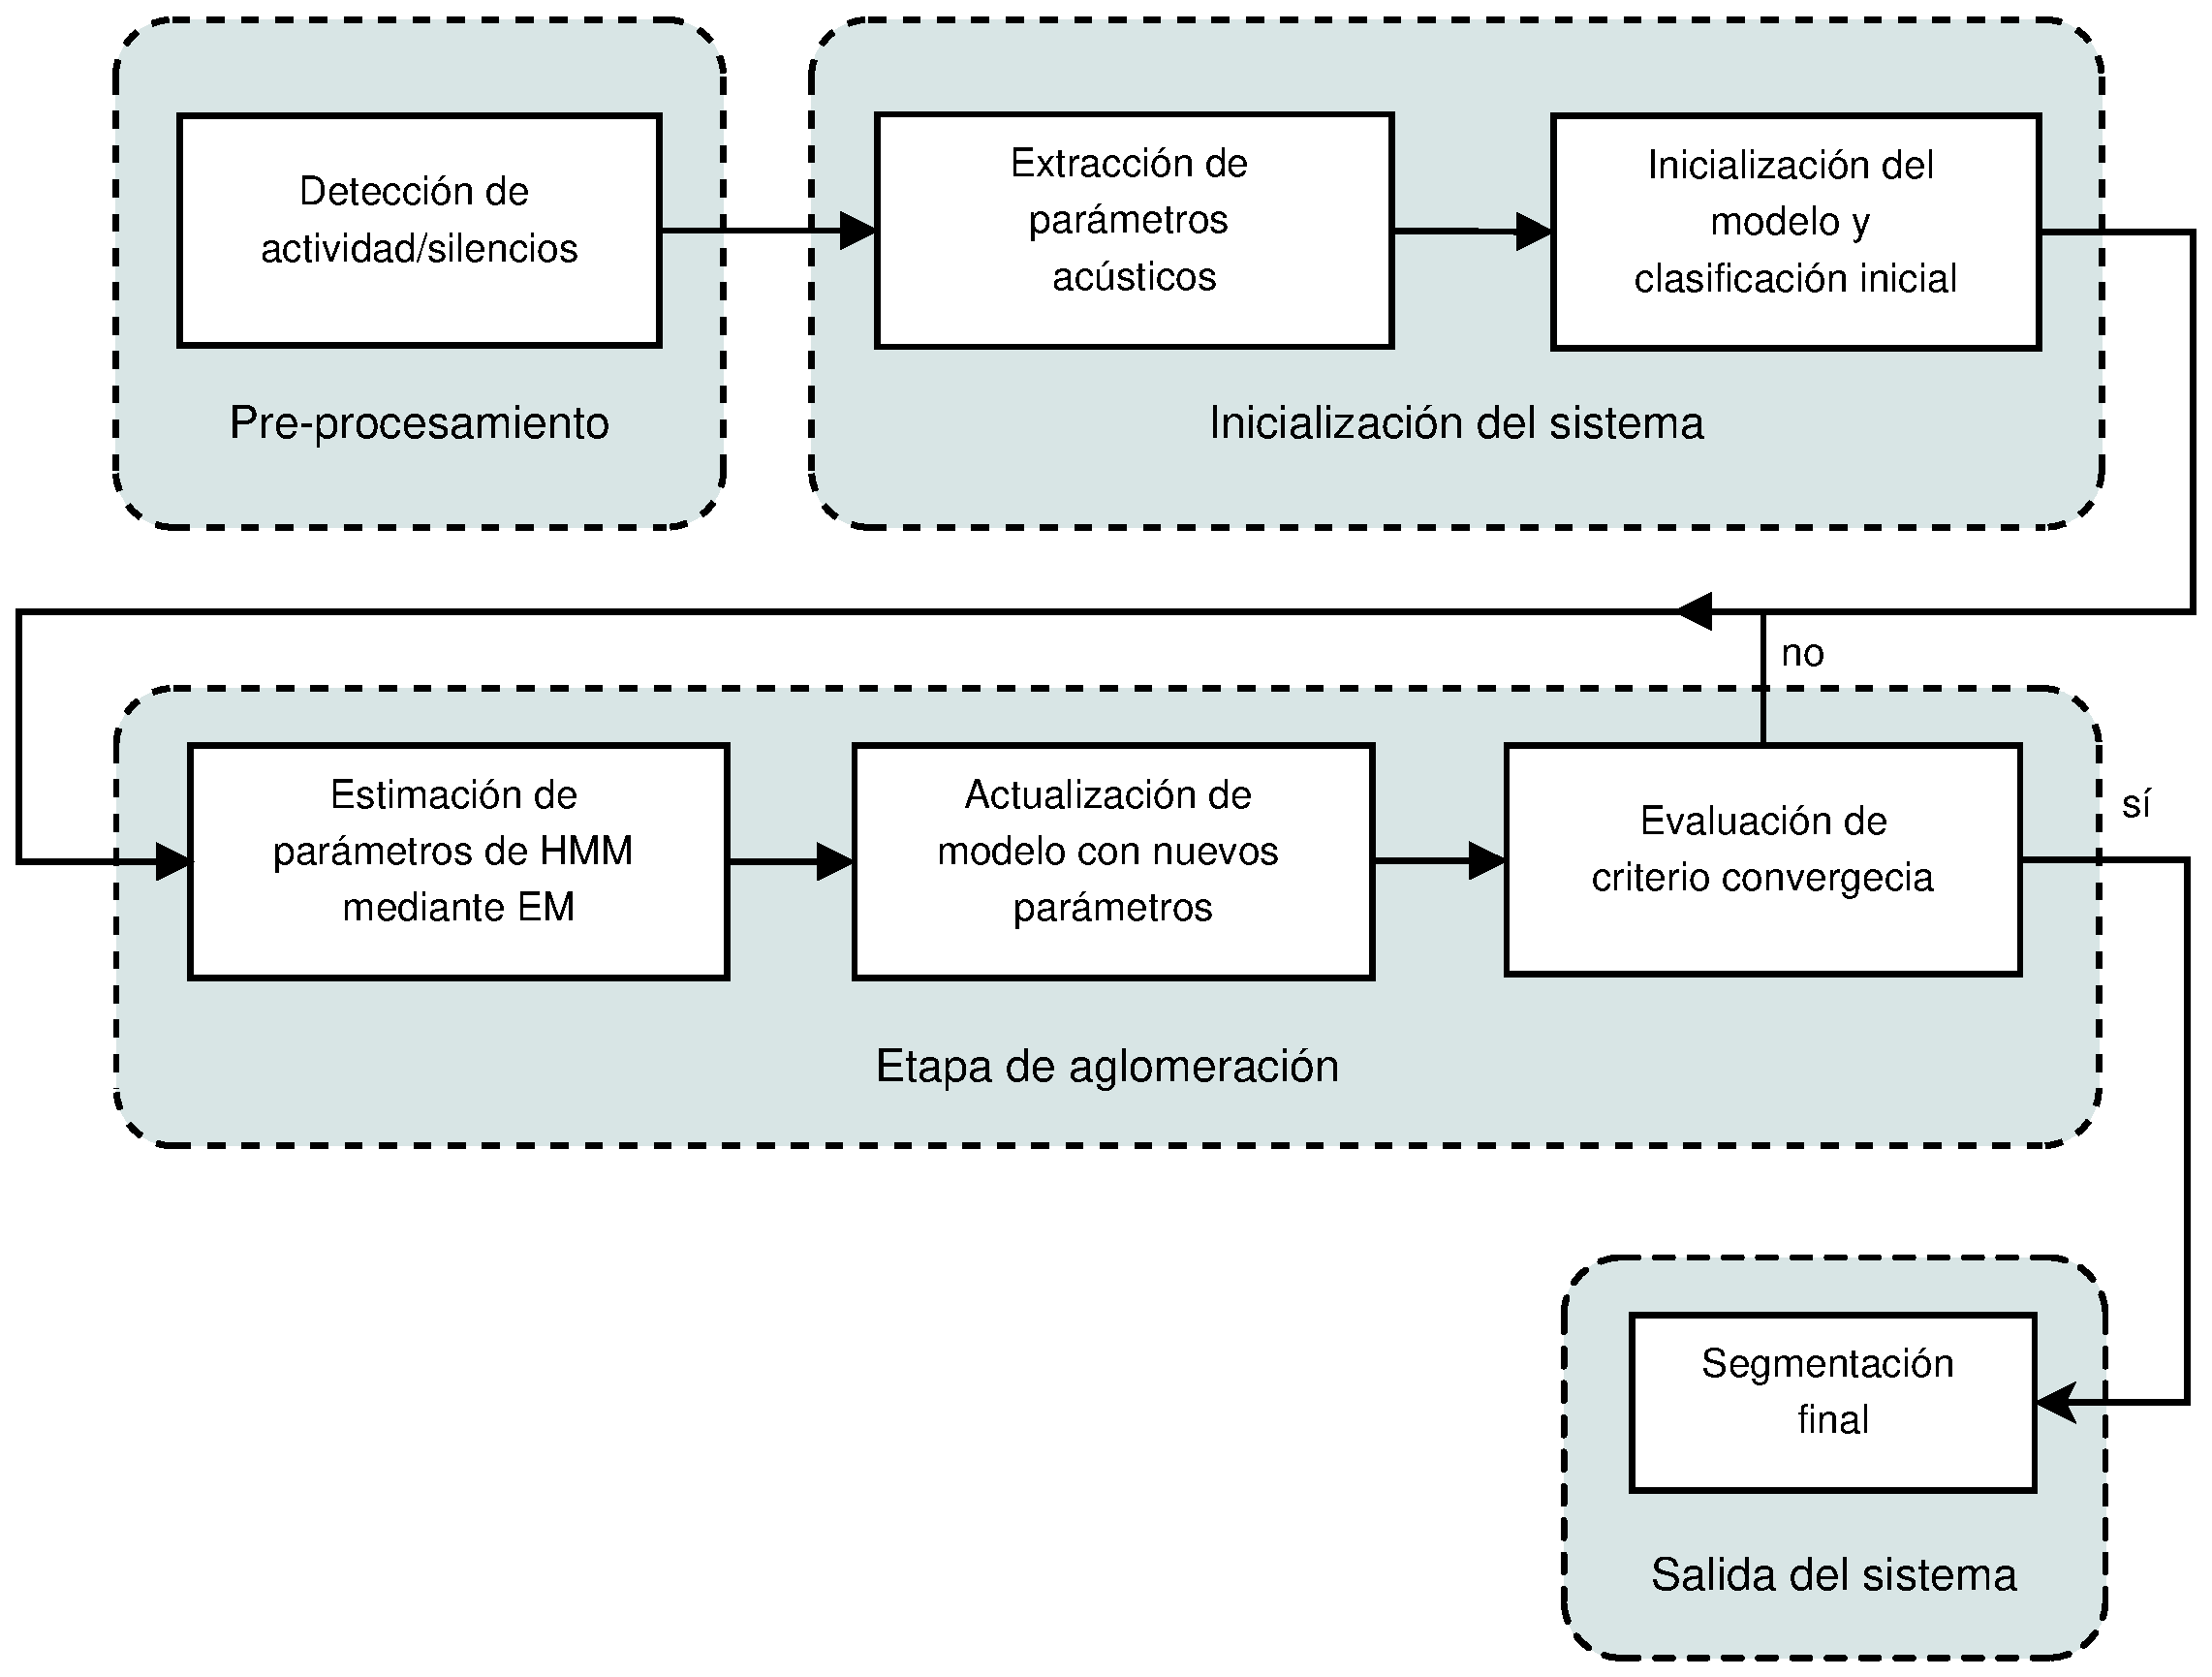
\includegraphics[width=1.4\linewidth]{gfx/chap2/ASR_flow}} \quad
  \caption[Esquema general del sistema.]{Esquema general del sistema. Se muestran las etapas principales para la estimación de la segmentación.}
  \label{fig:esquema}
\end{figure}


\section{Procesamiento acústico}

Antes de abordar de lleno el problema de \sd, se tiene que realizar cierto tratamiento a la señal de audio con la que se trabajará. 

Es decir, a partir de la señal de entrada (que se considerará es digital) se tratarán de obtener vectores de características cada cierto tiempo, que representen de forma adecuada los rasgos que nos interesan distinguir.

Una vez que se tienen estos vectores, se les aplica un algoritmo de aglomeración para entonces obtener un conjunto de etiquetas que se podrían considerar como posibles estados o palabras de diccionario referentes a la señal de audio.

El proceso en detalle se especifica a continuación: 

\subsection{Pre-procesamiento de señal de audio}

Se considera que se tiene una señal digital de voz, y que a partir de ésta se identificarán a las diferentes personas que hablan durante la grabación.

\begin{figure}[ht]
  {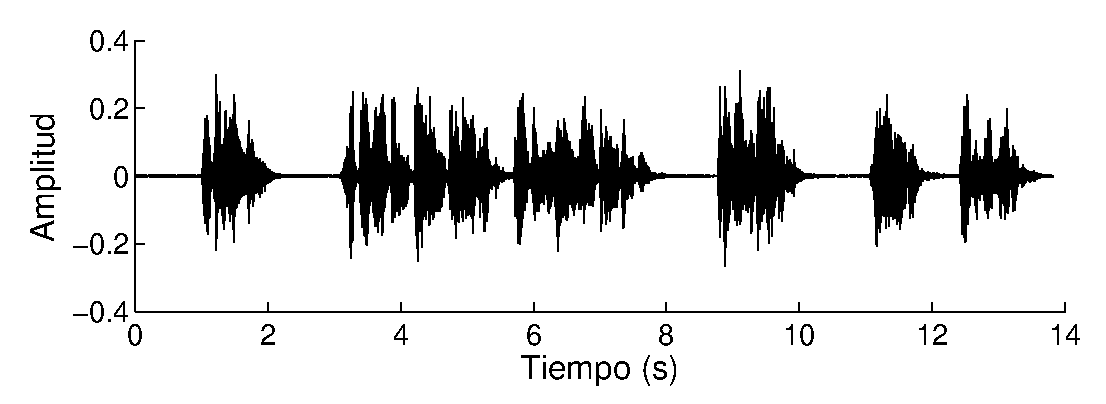
\includegraphics[width=0.9\linewidth]{gfx/chap2/signal0}} \quad
  \caption{Señal original de audio.}
  \label{fig:sign_orig}
\end{figure}

El primer paso en el procesamiento de la señal, es tanto la detección como eliminación de silencios; pues éstos realmente no nos interesan para la modelación del sistema. A esta etapa de pre-procesamiento se le suele conocer como \ac{SAD}.

\graffito{Nota: Tanto en ancho de la ventana, como el umbral del \ac{SAD} se pueden ajustar dependiendo de las características de la señal.}

Para realizar entonces la detección de los silencios, en esta primer etapa y como un primer intento para la eliminación de silencios, se hace una detección básica de qué partes de la señal son mayormente silencios.

Para ésto, se utiliza una ventana móvil que se irá recorriendo a lo largo señal, y que irá calculando el total de energía de la señal dentro de la ventana. Se considerará entonces silencio aquellas partes de la señal cuyo amplitud total esté debajo de un umbral específico.

A partir de esta ventana se podrán diferencias las partes que se tratarán como silencio de las partes que serán la señal resultante.

Como ya se mencionó, esta es una forma sencilla aunque no muy robusta de detectar en qué partes de la señal hay actividad. En otros trabajos, como 
en el de Istrate~et~al.~\cite{Istrate2005}, se presenta una etapa de \ac{SAD} mucho más profunda y diseñada para funcionar en entornos con múltiples micrófonos y proponen entrenar un modelo \ac{GMM} que sirva como clasificador luego para los silencios; que si bien muestra varias ventajas, está fuera del alcance de este trabajo.

\begin{figure}[ht]
  \begin{subfigure}[b]{\textwidth}
    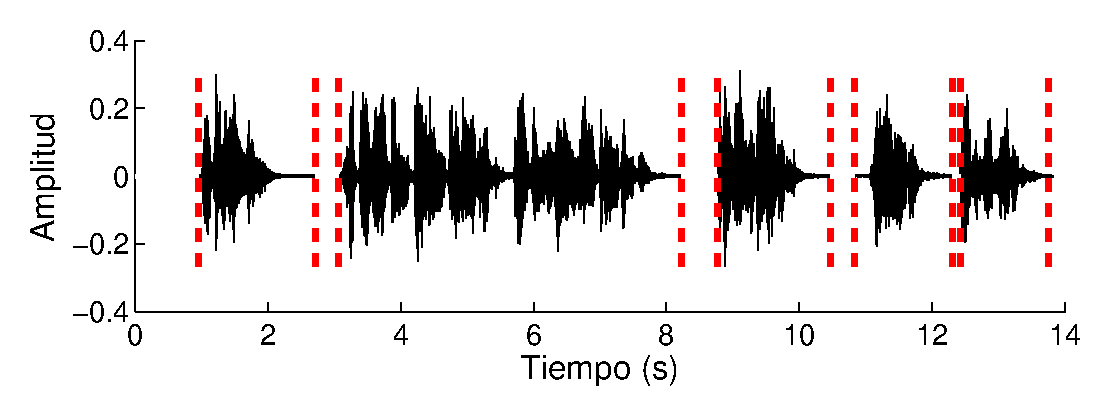
\includegraphics[width=0.9\linewidth]{gfx/chap2/signal1}
    \caption{Señal original con silencio identificado.}
    \label{fig:sign_silence}  
  \end{subfigure}

  \begin{subfigure}[b]{\textwidth}
    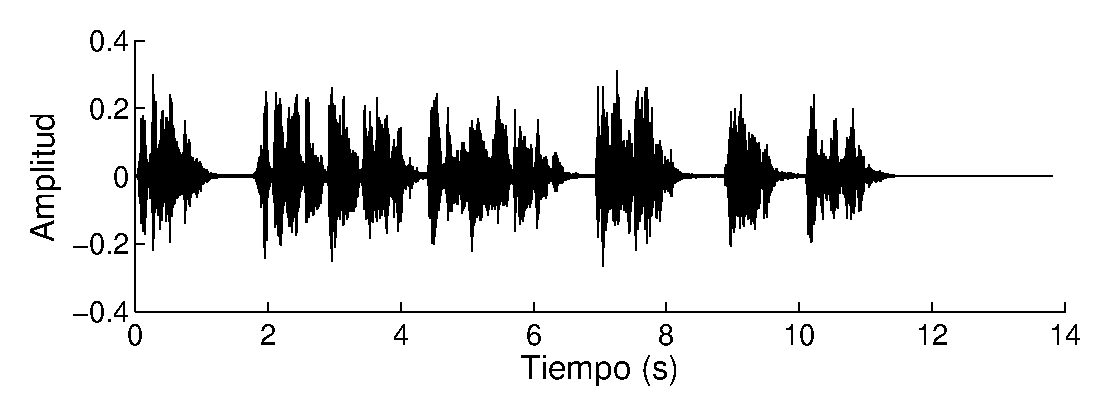
\includegraphics[width=0.9\linewidth]{gfx/chap2/signal2}
    \caption{Señal procesada y recortada.}
    \label{fig:sign_trunc}  
  \end{subfigure}
  
  \caption[Identificación/eliminación de silencios.]{Identificación y eliminación de silencio en señal.}  
  \label{fig:sign_ident}  
\end{figure}

Como se observa en la \autoref{fig:sign_trunc} basta entonces con eliminar los segmentos que contienen baja energía y reagrupar los segmentos restantes.

Con esto, se obtiene una señal en general más pequeña, y que se podría  considerar sólo contiene realmente los datos que se desea modelar.

\subsection{Obtención de características acústicas}

Una vez que se tiene la señal ya sin silencios, se trata de buscar características propias de la señal de audio que nos permitan identificar de buena forma los cambios de voz a través de la señal.

Tanto la extracción como selección de la mejor representación paramétrica de la señal de audio es una importante tarea en el diseño de cualquier sistema relacionado al reconocimiento o procesamiento de señales de audio. 

Para la tarea de \sd, se usarán los \ac{MFCC}, que son ampliamente utilizados por ejemplo en \sd~ entre otros procesos relacionados al procesamiento de voz; cuyo objetivo es comprimir la señal de audio eliminando la información que no es útil para análisis fonético.

Cabe mencionar, que originalmente los \ac{MFCC} fueron utilizados para la tarea específica de reconocimiento de voz por Davis~y~Mermelstein~\cite{Davis1980}, por lo que al momento de diseñarlos se trataba principalmente de que palabras iguales fueran parametrizadas de la misma manera sin importar quién la pronunciara. 

Esto va en contra del proceso requerido en \sd, puesto que se desea identificar a las diferentes personas que hablan, sin dar tanta importancia a qué es lo que están diciendo; por lo que la tarea de segmentación de señales de audio se vuelve un poco más complicada.

Para calcular los \ac{MFCC}, se usa la Escala de Frecuencia Mel, que está espaciada de forma lineal en frecuencias bajas, mientras que aumenta su separación de forma logarítmica para frecuencias más altas. Este cambio de separación se realiza comúnmente a partir de los $1000Hz$. 

A partir de esta escala, se diseña un banco de filtros triangulares que después se usará para construir un espectrograma de la señal (Ver \autoref{fig:sign_melfb}). Puesto que el banco de filtros de Mel trabajan en la frecuencia; a la señal de audio se le calcula la \ac{FT} y entonces a ésta es a quien se le aplica el banco de filtros.

\begin{figure}[t]
  \myfloatalign
  {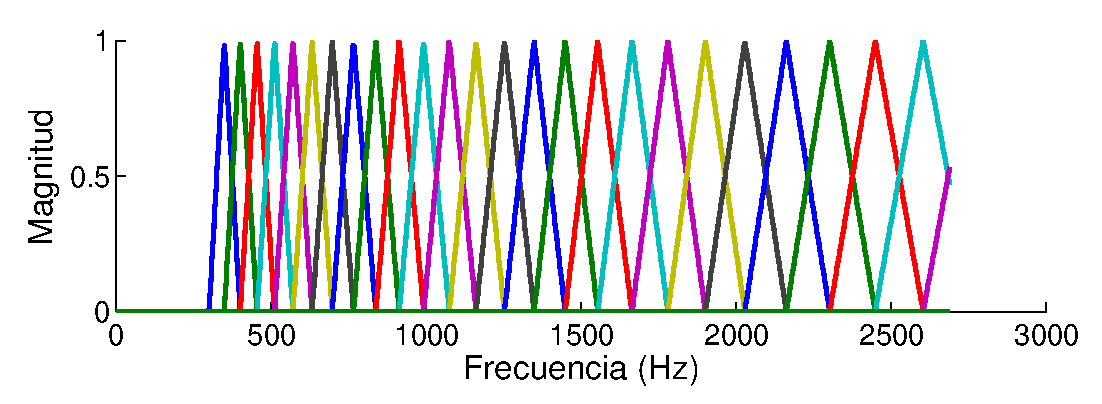
\includegraphics[width=0.9\linewidth]{gfx/chap2/mfcc_filterbank}} \quad
  \caption{Banco de filtros triangulares en frecuencia Mel.}
  \label{fig:sign_melfb}
\end{figure}  

Sea pues \autoref{fig:sign_trunc} la señal procesada sin los silencios, la respuesta que se obtiene al aplicar la \ac{FFT} y luego el banco de filtros de \autoref{fig:sign_melfb} se puede observar en la figura \autoref{fig:sign_melres}.

Para ser más específicos, la operación que se utiliza para construir el espectrograma es en realidad la \ac{STFT}; que si bien está basada en una \ac{FT}, se aplica de forma separada a segmentos de la señal de audio. 

Se puede pensar como una secuencia de operaciones \ac{DCT} por segmentos usando una ventana movible. Como menciona Rabiner~y~Schafer~\cite{Rabiner2007}, este método es la base en la mayoría de las técnicas relativas a procesamiento de voz, pues la construcción de un espectrógrama permite de forma sencilla analizad (y visualizar) la respuesta de una señal a un cierto banco de filtros entonado a alguna frecuencia.

Esto permite definir una resolución específica con la que se trabajará, dependiendo de las características que se desean obtener. Por ejemplo, si se desea que la respuesta tenga una mejor resolución en frecuencia, se debería usar un tamaño de ventana mayor, en relación a la periodicidad de la señal; aunque esto implicará que se pierda sensibilidad en la dimensión del tiempo. Por otro lado, si se utiliza una ventana de tamaño menor, la respuesta será mucho más precisa en cuanto al tiempo, pero se la resolución en frecuencia será más burda \cite{Rabiner1993}.

\begin{figure}[t]
  \myfloatalign
  {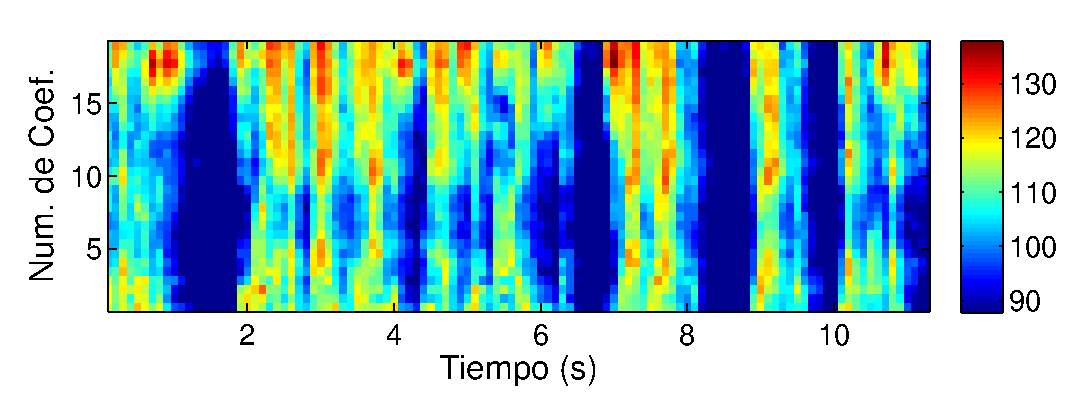
\includegraphics[width=0.9\linewidth]{gfx/chap2/mfcc_result2}} \quad
  \caption{Respuesta al banco de filtros.}
  \label{fig:sign_melres}
\end{figure}

La matriz que se muestra en \autoref{fig:sign_melres} corresponde a la respuesta al banco de filtros. Cada renglón representa la frecuencia a la que está entonado un filtro en específico del banco; mientras que cada columna indica la muestra en tiempo en que se analiza la señal. Por último, la intensidad en la escala de colores es la respuesta al banco de filtros, o la amplitud con la que cada frecuencia se presenta en cierto momento.

La dimensión de esta matriz dependerá de la misma construcción del banco de filtros (tanto el número de canales que se usarán, como el tamaño de ventana que se usará para las convoluciones); pero en general se obtendrán matriz de gran tamaño; por lo que es conveniente tratar de disminuir la dimensionalidad de estos datos.

Para esto, a la respuesta obtenida del banco de filtros se le aplicará la \ac{DCT}, para tratar de concentrar la energía en ciertos componentes (los primeros $n$ coeficientes), y descartar los restantes. A esta etapa se le conoce como extracción de los coeficientes cepstrales. 

\begin{algorithm}[bt]
   \caption{\textit{MFCC}}
   \label{alg:mfcc}
\begin{algorithmic}
   \STATE {\bfseries Input:} \\ Señal digital $\lbrace s_n \rbrace_1^T $,
   \STATE Iniciar $\mu_{1:k} = sample(x_{1:N}, K)$   
   
   \STATE $t = 0$
   \STATE $l_{1:N}^{(t)} = 0$
      
   \REPEAT  
   \STATE $t=t+1$ 
   \STATE $l_n^{(t)} = \text{arg min}_k {\left \| x_n - \mu_k \right \|}^2 $
   \STATE $r_{nk}$ = $\mathbbm{1}_k\left(l_n^{(t)}\right)$
   \STATE $\mu_k = \left\lbrace {\sum_{n=1}^N r_{nk} x_n} \right\rbrace / \left\lbrace {\sum_{n=1}^N r_{nk}} \right\rbrace $
   \UNTIL{$l^{(t)}$ == $l^{(t+1)}$}
\end{algorithmic}
\end{algorithm}

Como ya se mencionó previamente, el banco de filtros utilizado está separado  en la frecuencia Mel, pues aproximan mucho mejor la respuesta del sistema auditivo humano que un banco de filtros linealmente espaciados \cite{Vyas2013}. 

Después de este proceso, nuestros datos se podrían representar de la siguiente manera (\autoref{fig:sign_mfcc}) que son los \ac{MFCC} que antes habíamos mencionado.
\begin{figure}[t]
  \myfloatalign
  {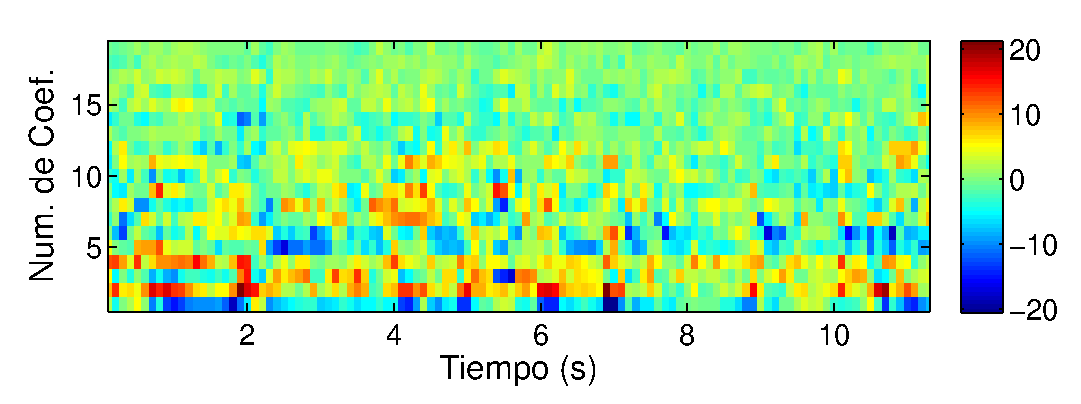
\includegraphics[width=0.9\linewidth]{gfx/chap2/mfcc_result3}} \quad
  \caption{Mel Frequency Cepstrum Coefficients.}
  \label{fig:sign_mfcc}
\end{figure}

Por último, para los modelos que usaremos, se necesitan que las características estén de cierta forma \textit{discretizadas}, es decir, no nos es útil el tener para cada observación en el tiempo un vector de características; sino que necesitamos una etiqueta o clase para cada observación. 

Para esto, podemos utilizar diferentes métodos tanto de reducción de dimensionalidad como de agrupación/clasificación. Como primer idea, utilizaremos el método de \textit{k-means} para agrupar los vectores de acuerdo a su cercanía en el espacio euclidiano.

Se tendría entonces el siguiente resultado para nuestra matriz de MFCC obtenida:
\begin{figure}[t]
  \myfloatalign
  {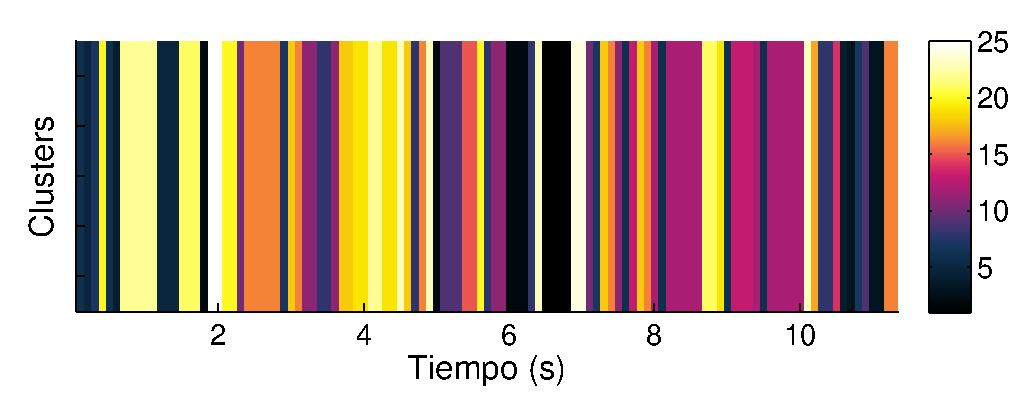
\includegraphics[width=0.9\linewidth]{gfx/chap2/mfcc_result4}} \quad
  \caption{MFCC agrupados con k-means++.}
  \label{fig:sign_clusters}
\end{figure}
Cabe aclarar que usamos una variante del algoritmo original de k-means, que se llama \textit{k-means++} \cite{Arthur2007} y que propone una mejor inicialización para que el algoritmo converja más rápido. En \autoref{alg:kmeanspp} se describe mejor esta etapa inicial.

\begin{algorithm}[bt]
   \caption{\textit{k-means}}
   \label{alg:kmeans}
\begin{algorithmic}
   \STATE {\bfseries Input:} \\ Conjunto de datos $\lbrace x_n \rbrace_1^N $, número de grupos $K$
   \STATE 
   \STATE Iniciar $\mu_{1:k} = sample(x_{1:N}, K)$   
   
   \STATE $t = 0$
   \STATE $l_{1:N}^{(t)} = 0$
      
   \REPEAT  
   \STATE $t=t+1$ 
   \STATE $l_n^{(t)} = \text{arg min}_k {\left \| x_n - \mu_k \right \|}^2 $
   \STATE $r_{nk}$ = $\mathbbm{1}_k\left(l_n^{(t)}\right)$
   \STATE $\mu_k = \left\lbrace {\sum_{n=1}^N r_{nk} x_n} \right\rbrace / \left\lbrace {\sum_{n=1}^N r_{nk}} \right\rbrace $
   \UNTIL{$l^{(t)}$ == $l^{(t+1)}$}
\end{algorithmic}
\end{algorithm}

\begin{algorithm}[bt]
   \caption{\textit{k-means++}}
   \label{alg:kmeanspp}
\begin{algorithmic}
   \STATE {\bfseries Input:} \\ Conjunto de datos $\lbrace x_n \rbrace_1^N $, número de grupos $K$
   \STATE 
   \STATE $\mu_{1} = sample(x_{1:N}, 1)$   
   \FOR{k:=2 \TO $K$} 
     \STATE $m_n = \text{arg min}_{\mu_j} {\left \| x_n - \mu_j \right \|}^2 
      ~~\forall~~ j = {1, ..., k-1}; ~n = {1, ..., N} $
     \STATE $D_{n} = dist(x_n, m_n) ~~\forall~~  n = {1, ..., N}$
     \STATE $p_{n} = D_{n}^2 ~~\forall~~  n = {1, ..., N}$
     \STATE $\mu_{k} = sample(x_{1:N}, 1, p_{1:N})$   
   \ENDFOR
   
   \STATE $t = 0$
   \STATE $l_{1:N}^{(t)} = 0$
      
   \REPEAT  
   \STATE $t=t+1$ 
   \STATE $l_n^{(t)} = \text{arg min}_k {\left \| x_n - \mu_k \right \|}^2$
   \STATE $r_{nk}$ = $\mathbbm{1}_k\left(l_n^{(t)}\right)$
   \STATE $\mu_k = \left\lbrace {\sum_{n=1}^N r_{nk} x_n} \right\rbrace / \left\lbrace {\sum_{n=1}^N r_{nk}} \right\rbrace $
   \UNTIL{$l^{(t)}$ == $l^{(t+1)}$}
\end{algorithmic}
\end{algorithm}

Ahora sí, con nuestro vector de etiquetas correspondiente a la señal de audio, se podrá aplicar un modelo y tratar de inferir los parámetros que le correspondan.


% section section_name (end)